\documentclass[../../main.tex]{subfiles}
\cite{germannwikipedia}
\cite{germannhistorischeslexikon}
\cite{germannpersonenlexikon}
\paragraph{}
\begin{figure}[h]
    \centering
    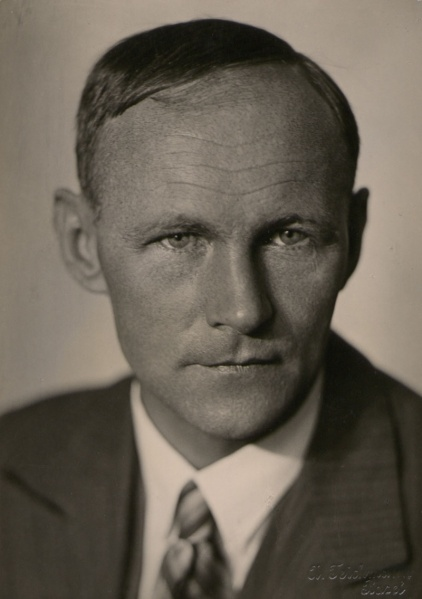
\includegraphics[width=\textwidth,height=7cm,keepaspectratio]{images/germann.jpg}
    \caption{Oscar Adolf Germann (unbekannt). personenlexikon.bl.ch. (23. Dezember 2014). \newline URL: https://personenlexikon.bl.ch/Datei:GermannO1889.jpg [Stand 16.07.2019]}
\end{figure}
Oscar Adolf Germann wurde am 19. August 1889 in Frauenfeld geboren. Sein Vater Adolf Germann war ein FDP-Politiker, seine Mutter hiess Hermine Germann. Oscar Germann hatte drei Brüder.
\paragraph{}
Germann besuchte die Kantonsschule in Frauenfeld, später studierte er Rechtswissenschaft in Zürich, dabei lehrte er einige Semester in Deutschland und Österreich. 1918 wurde er als Experte im Eidgenössischen Volkswirtschaftsdepartement angestellt. Zehn Jahre später, 1928, wurde er Professor für Arbeitsrecht an der Universität Bern. Von 1930 bis 1960 war er Professor für Strafrecht an der Universität Basel.
\paragraph{}
Nebst seinen Tätigkeiten als Professor hatte Germann eine Karriere im Militär. 1923 wurde er Generalstabsoffizier der Schweizer Armee, 1937 wurde er Stabschef des zweiten Armeekorps. Von 1939 – 1940 war er Mitarbeiter und zeitweise Leiter der Operationssektion im Armeestab. Während dieser Zeit erarbeitete Germann die Aufmarschpläne Nord und West, welche eine Zusammenarbeit mit der französischen oder deutschen Armee beinhalteten. Germann erstellte den Rückzugsplan in die Wiggerstellung. Germann war zudem ein Befürworter der Reduit-Strategie und verfasste einen der beiden Reduit-Strategie-Pläne. Der Plan von Samuel Gonard wurde dem seinigen jedoch vorgezogen, weshalb Germanns Plan schliesslich nie ausgeführt wurde. Von 1941 – 1944 war Germann Stabschef des 4. Armeekorpses. 1945, noch vor dem Ende des zweiten Weltkrieges, beendete Germann seine militärische Laufbahn.
\paragraph{}
Germann war verheiratet mit Elisabeth Martin, mit ihr hatte er zwei Töchter und einen Sohn. Im hohen Alter von 90 Jahren verstarb Oscar Adolf Germann in Bottmingen, einer Gemeinde im Kanton Basel-Landschaft.